\documentclass{beamer}
\usepackage[utf8]{inputenc}
\usepackage{graphicx}
\usepackage[justification=centering]{caption}
\usepackage{hyperref}
\usepackage{url}
\usepackage{amsmath}
\usepackage{amssymb}
\usepackage{bm}
\usepackage{pgfplots}

\DeclareMathOperator{\sign}{sign}

\usetheme[sectionpage=progressbar, progressbar=frametitle]{metropolis}
\setbeamertemplate{section in toc}{\inserttocsectionnumber.~\inserttocsection}

\title{Fundamentals of Neural Networks}
\date{\today}
\author{Mathias Jackermeier}
\institute{Technische Universität München}
\begin{document}
	\maketitle
	\begin{frame}{Introduction}
	\begin{figure}
		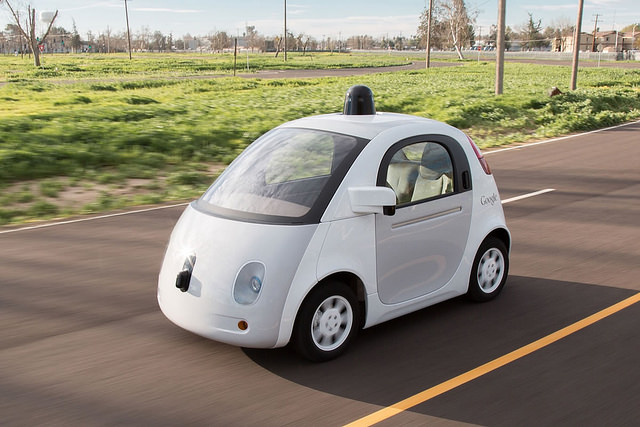
\includegraphics[scale=.4]{img/self_driving}
		\caption{A self-driving car. \\Credit: 
			\href{https://www.flickr.com/photos/chijs/21798665468/in/photolist-zdgRMN-HzGNh8-gTzd3u-o5Zrtr-dLznp8-rntpFL-FnbXbs-Hap7Do-9o1FrD-GE5zz3-G9tVGQ-GhD21n-eb2sof-cDdb3y-Gfm7Po-NZGQ3J-GEawvr-FSwEH9-Fnc15o-zhGLV-GbMR1r-FnnkQp-Gfm7CG-eE2tFc-GbMRjx-GbMSe8-9mUNbt-CJdtas}{Marc van der Chijs}
			 / \href{https://creativecommons.org/licenses/by-nd/2.0/}{CC BY-ND 2.0}}
	\end{figure}
	\end{frame}
	\begin{frame}{Introduction}
		\begin{figure}
			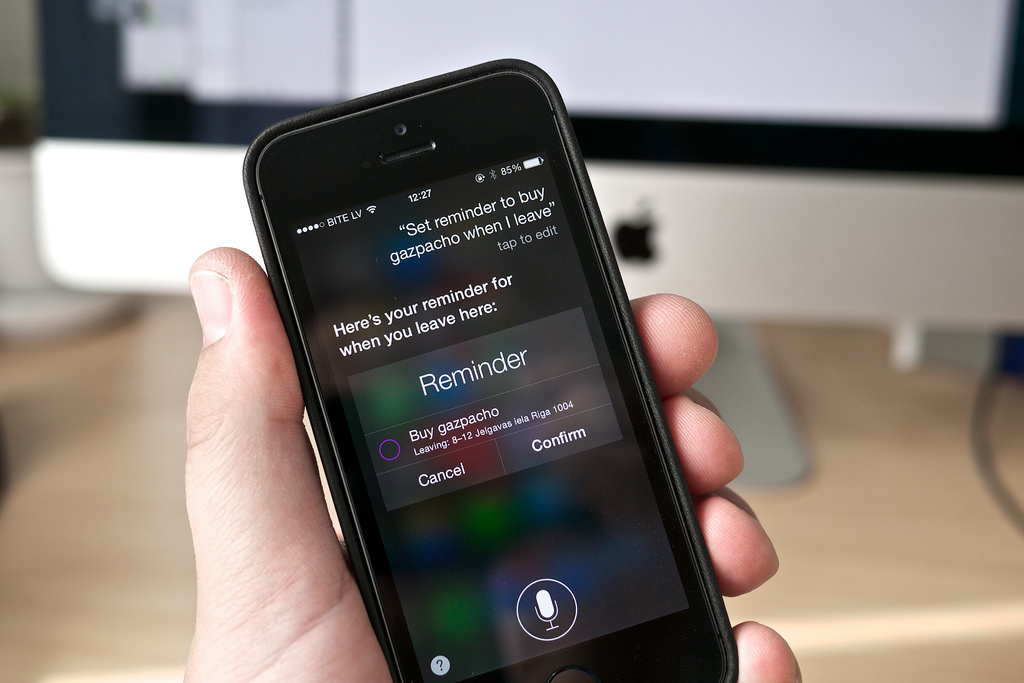
\includegraphics[scale=.25]{img/siri}
			\caption{A digital assistant. \\Credit: 
				\href{https://www.flickr.com/photos/65265630@N03/13989720008}{Kārlis Dambrāns} / \href{https://creativecommons.org/licenses/by/2.0/}{CC BY 2.0}}
		\end{figure}
	\end{frame}
	%Jedes intelligente System benutzt neuronale Netze
	\section{Outline}
	\section{The Perceptron}
	\begin{frame}{Example Task}
		\begin{itemize}
			\item<1-> Predict whether an input image of a handwritten digit shows a zero or another digit
		\end{itemize}
	\end{frame}
	\begin{frame}{MNIST Data Sample}
		\begin{figure}
			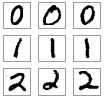
\includegraphics[scale=1.6]{img/mnist}
			\caption{Examples from the {MNIST} database. \\Credit: 
				\href{https://commons.wikimedia.org/wiki/File:MnistExamples.png}{Josef Steppan}
				/ \href{https://creativecommons.org/licenses/by-sa/4.0/deed.en}{CC BY-SA 4.0}}
		\end{figure}
	\end{frame}
	\begin{frame}{Example Task}
		\begin{itemize}
			\item <1-> Predict whether an input image of a handwritten digit shows a zero or another digit
			\item <1-> The image is represented as a flattened vector of pixel intensities $\bm{x} \in \mathbb{R}^{784}$
			\item <2-> The output should be $1$ if the image shows a zero, otherwise it should be $-1$
			\item <3-> \textbf{Idea}: Assign a weight to every input pixel
		\end{itemize}
	\end{frame}
	\begin{frame}{Model Specification}
		The perceptron accepts $n$ input values and computes an output value $\hat{y}$:
		\begin{equation}
			\begin{split}
			\hat{y} &= \sign\left (\sum_{i=1}^{n} w_ix_i\right )\\
			\equiv \hat{y} &= \sign\left (\bm{w}^\top\bm{x}\right )
			\end{split}
		\end{equation}
	\end{frame}
	% Jedem Pixel wird ein Gewicht zugeordnet
	% z.B.: Mitte negativ, bei der 0 positiv
	\begin{frame}{Visual Representation}
		\begin{figure}
			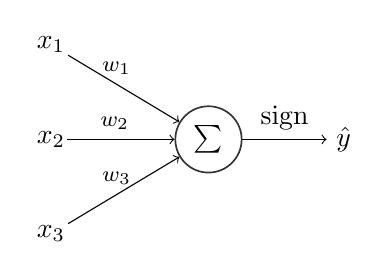
\begin{tikzpicture}
	\tikzstyle{neuron} = [circle,draw=black!80,semithick,minimum size=20pt]
	% input layer
	\foreach \i in {1,...,3}
		\node (input\i) at (0, -\i*1.2) {$x_\i$};
	% perceptron
	\node[neuron] (perceptron) at (2, -2*1.2) {$\sum$};
	% connections
	\foreach \i in {1,...,3}
		\draw[->, shorten <= -.1cm] (input\i) -- node[pos=.4,above]{\footnotesize{$w_\i$}} (perceptron);
	% output
	\draw[->] (perceptron) -- node[above]{$\sign$}(3.5, -2*1.2) node[right]{$\hat{y}$};
\end{tikzpicture}
			\caption{A visual representation of the perceptron model.}
		\end{figure}
	\end{frame}
	% Based on neuroscience
	\begin{frame}{Generalizations}
		\begin{itemize}
			\item <1-> The perceptron is often used in a modified form
			\item <2-> A scalar bias value can be added to the output computation:
			\begin{equation}
			\hat{y} = \sign\left (\bm{w}^\top\bm{x} + b\right )
			\end{equation}
			\item <3-> The $\sign$ function can be replaced with a generic function $f$:
			\begin{equation}
			\hat{y} = f\left (\bm{w}^\top\bm{x} + b\right )
			\end{equation}
			\item <4> These modified perceptrons are often called \emph{neurons} or simply \emph{units}
		\end{itemize}
	\end{frame}
	\begin{frame}{Shortcomings of the Perceptron}
		\begin{figure}
			% !TeX root = template_Beamer.tex

% restrict y to domain=-1:1, x=1cm
\begin{tikzpicture}[scale=.9]
	\begin{axis}[axis lines = left,xlabel = $x_1$, ylabel = {$x_2$}, ymin=-0.1, ymax=1.1, mlineplot, xmin=-0.1, xmax=1.1]
		\addplot[mark=o,mark size=5pt] coordinates {(0,1)};
		\addplot[mark=o,mark size=5pt] coordinates {(1,0)};
		\addplot[mark=x,mark size=5pt] coordinates {(0,0)};
		\addplot[mark=x,mark size=5pt] coordinates {(1,1)};
	\end{axis}
\end{tikzpicture}			
			\caption{The perceptron cannot learn the \textsc{xor} function since the data is not linearly separable.}
		\end{figure}
	\end{frame}
	
	\section{Feedforward Neural Networks}
	
	\begin{frame}{Networks of perceptron-like units}
		\begin{itemize}
			\item <1-> \textbf{Idea}: A combination of multiple perceptrons could make much better predictions
			\item <2-> We arrange the perceptrons in layers
			\item <3-> The input of a layer is the output of the previous layer
			\item <4-> This network model is called \emph{feedforward neural network} or \emph{multilayer perceptron}
		\end{itemize}
	\end{frame}
	% Angelehnt an Gehirn
	
	\begin{frame}{Visual Representation}
		\begin{figure}
			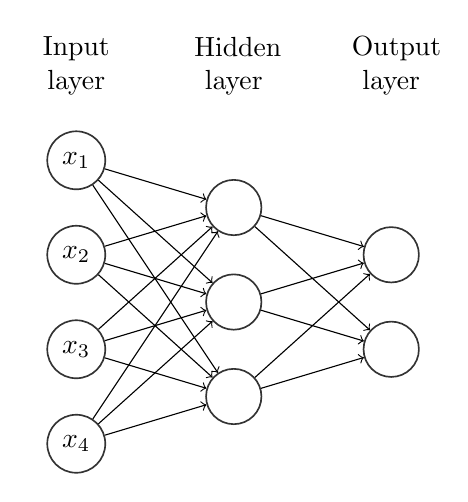
\begin{tikzpicture}
	\tikzstyle{neuron} = [circle,draw=black!80,semithick,minimum size=20pt]
	\tikzstyle{layer} = [text width=1cm, align=center]
	% input layer
	\node[layer] at (0, 0) {Input layer};
	\foreach \i in {1,...,4}
		\node[neuron] (input\i) at (0, -\i*1.2) {$x_\i$};
	% hidden layer
	\node[layer] at (2, 0) {Hidden layer};
	\foreach \i in {1,...,3}
		\node[neuron] (hidden\i) at (2, -\i*1.2 -.6) {};
	% output layer
	\node[layer] at (4, 0) {Output layer};
	\foreach \i in {1,...,2}
		\node[neuron] (output\i) at (4, -\i*1.2 -1.2) {};
	% connections input->hidden
	\foreach \i in {1,...,4}
		\foreach \j in {1,...,3}
			\draw[->] (input\i) -- (hidden\j);
	% connections hidden->output
	\foreach \i in {1,...,3}
		\foreach \j in {1,...,2}
			\draw[->] (hidden\i) -- (output\j);
\end{tikzpicture}
			\caption{A three-layer feedforward neural network.}
		\end{figure}
	\end{frame}
	
	\begin{frame}{Mathematical Formulation}
		\begin{itemize}
			\item <1-> We can specify a single neuron with a weight vector $\bm{w}$ and a bias value $b$
			\item <2-> Since a neural network consists of multiple neurons in a layer, we need weight \emph{matrices} $\bm{W}^{(l)}$ and bias \emph{vectors} $\bm{b}^{(l)}$ to specify the parameters of a layer $l$
			\item <3-> The weight $w_{ij}^{(l)}$  is the weight from the xx neuron in the xx layer to the xx neuron in the xx layer
			\item <4-> The bias $b_i^{(l)}$ is the bias of the xx neuron in the xx layer
		\end{itemize}
	\end{frame}
	
	\begin{frame}{Mathematical Formulation}
		\begin{itemize}
			\item <1-> The output at layer $l$ is then given by
			\begin{equation}
				\bm{a}^{(l)} = f^{(l)}\left(\bm{W}^{(l)\top}\bm{a}^{(l-1)}+\bm{b}^{(l)}\right)
			\end{equation}
		\end{itemize}
	\end{frame}
	% TODO: überall left mit den Klammer machen
	
	\subsection{Architecture}
	\subsection{Mathematical formulation}
	\section{Training Feedforward Neural Networks}
	\subsection{Cost functions}
	\subsection{Stochastic Gradient Descent}
	\subsection{Back-propagation}
	\section{Extensions}
	
	\begin{frame}[standout]
	Thank you!
	\end{frame}
	
\end{document}